\documentclass[tikz,border=3pt,10pt]{standalone}
\usepackage{fontspec}
\setmainfont{STIXTwoText-Regular.otf}[
    Path=../../../../../../../assets/fonts/,
    BoldFont=STIXTwoText-Bold.otf,
    ItalicFont=STIXTwoText-Italic.otf,
    BoldItalicFont=STIXTwoText-BoldItalic.otf
]
\usepackage{unicode-math}
\setmathfont{STIXTwoMath.otf}[Path=../../../../../../../assets/fonts/]
\usepackage{pgfplots}
\pgfplotsset{compat=1.18}
\usetikzlibrary{backgrounds, intersections, patterns, arrows.meta}

% BEGIN ZO MATH GRAPH STYLE — VERSION 05 — 2026-07-30
% Copy this block verbatim into every graph source.

\definecolor{zoWhite}{HTML}{FFFFFF}
\definecolor{zoPlotBackground}{HTML}{FFF9E9}
\definecolor{zoPlotBorder}{HTML}{DFD7CA}
\definecolor{zoBackground}{HTML}{FBFAF8}
\definecolor{zoGridMinor}{HTML}{F8F5F0}
\definecolor{zoGridMajor}{HTML}{DFD7CA}
\definecolor{zoAxis}{HTML}{554F48}
\definecolor{zoText}{HTML}{3E3A35}
\definecolor{zoTextStrong}{HTML}{25221F}
\definecolor{zoGraphMain}{HTML}{EF5350}
\definecolor{zoGraphStrong}{HTML}{BF4240}
\definecolor{zoGraphSecondary}{HTML}{997918}
\definecolor{zoReference}{HTML}{997918}
\definecolor{zoHighlight}{HTML}{FFCA28}
\definecolor{zoHighlightLight}{HTML}{FFF4D4}
\definecolor{zoSuccess}{HTML}{1DE8B5}

\pgfplotsset{
  zo axis/.style={
    width=12cm,
    height=7.5cm,
    scale only axis,
    axis equal image=false,
    enlargelimits=false,
    clip=true,
    clip mode=individual,
    axis lines=middle,
    grid=none,
    axis line style={draw=zoAxis,line width=0.8pt,<->},
    tick align=center,
    tickwidth=0.4mm,
    tick style={draw=zoAxis,line width=0.32pt},
    every axis x label/.append style={
      text=zoText,
      font=\normalsize
    },
    every axis y label/.append style={
      text=zoText,
      font=\normalsize
    },
    every tick label/.append style={
      text=zoText,
      font=\footnotesize
    },
    every axis plot/.append style={line cap=round,line join=round}
  },
  zo grid/.style={
    major grid style={draw=zoGridMajor,line width=0.35pt},
    minor grid style={draw=zoGridMinor,line width=0.25pt}
  },
  zo graph main/.style={
    draw=zoGraphMain,
    line width=1.2pt,
    solid,
    no marks
  },
  zo graph secondary/.style={
    draw=zoGraphSecondary,
    line width=0.9pt,
    solid,
    no marks
  },
  zo graph strong/.style={
    draw=zoGraphStrong,
    line width=1.2pt,
    solid,
    no marks
  },
  zo reference/.style={
    draw=zoReference,
    line width=0.6pt,
    dashed,
    no marks
  },
  zo asymptote/.style={
    draw=zoReference,
    line width=0.8pt,
    dashed,
    no marks
  },
  zo auxiliary line/.style={
    draw=zoAxis,
    line width=0.6pt,
    densely dashed,
    no marks
  },
  zo point closed/.style={
    only marks,
    mark=*,
    mark size=2.2pt,
    draw=zoGraphMain,
    fill=zoGraphMain
  },
  zo point open/.style={
    only marks,
    mark=*,
    mark size=2.2pt,
    draw=zoGraphMain,
    fill=zoPlotBackground,
    line width=0.8pt
  },
  zo point emphasized/.style={
    only marks,
    mark=*,
    mark size=2.8pt,
    draw=zoGraphStrong,
    fill=zoGraphStrong
  },
  zo point auxiliary/.style={
    only marks,
    mark=*,
    mark size=1.7pt,
    draw=zoReference,
    fill=zoReference
  }
}

\tikzset{
  zo graph field/.style={
    show background rectangle,
    inner frame sep=4mm,
    background rectangle/.style={
      fill=zoPlotBackground,
      draw=zoPlotBorder,
      line width=0.45pt,
      rounded corners=2mm
    }
  },
  zo axis label/.style={
    text=zoText,
    font=\normalsize
  },
  zo origin label/.style={
    text=zoText,
    font=\normalsize
  },
  zo graph label/.style={
    text=zoText,
    font=\small
  },
  zo annotation box/.style={
    fill=zoWhite,
    draw=zoPlotBorder,
    line width=0.45pt,
    rounded corners=1mm,
    inner sep=5pt
  }
}
% END ZO MATH GRAPH STYLE

\begin{document}
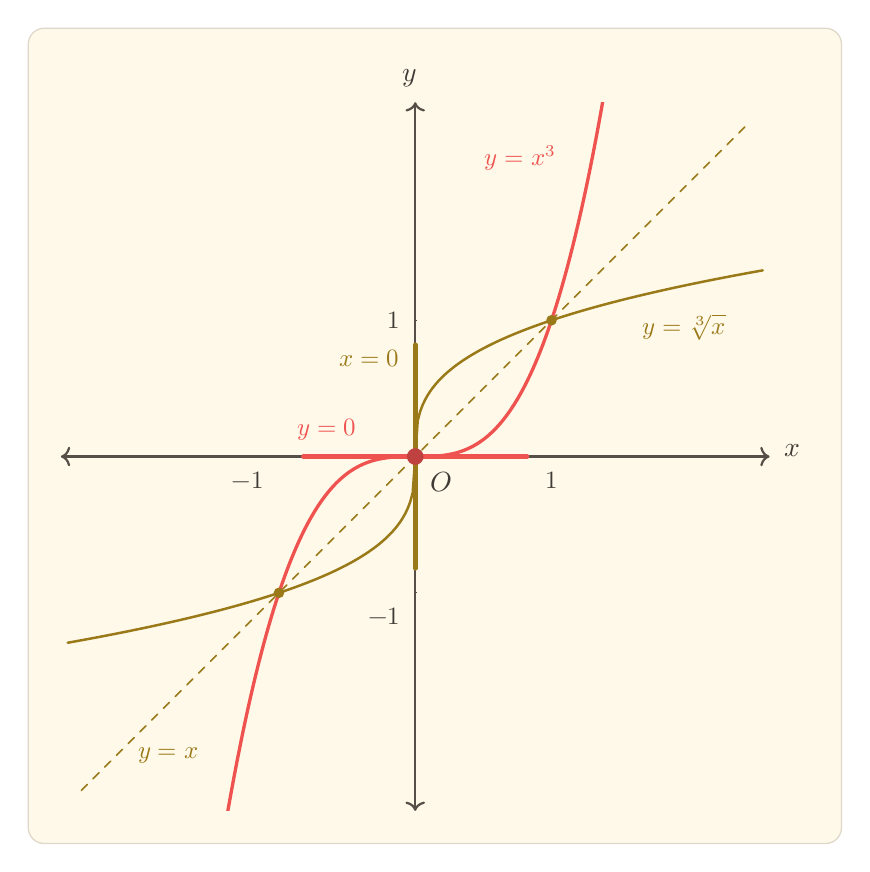
\begin{tikzpicture}[zo graph field]
\begin{axis}[
    zo axis,
    width=9cm,
    height=9cm,
    axis equal image=true,
    xmin=-2.6, xmax=2.6,
    ymin=-2.6, ymax=2.6,
    xtick={-1,1},
    xticklabel=\empty,
    ytick={-1,1},
    yticklabel=\empty,
    xlabel={$x$},
    ylabel={$y$},
    xlabel style={anchor=west, xshift=2pt, yshift=2pt},
    ylabel style={anchor=south, xshift=-2pt, yshift=2pt}
]

    % Reflection axis
    \addplot[zo reference, domain=-2.45:2.45, samples=2] {x};

    % Main function y=x^3, clipped to the observation window
    \addplot[zo graph main, domain=-1.375:1.375, samples=180] {x^3};

    % Inverse function y=cuberoot(x), split at 0 for robust real-valued sampling
    \addplot[zo graph secondary, domain=0:2.55, samples=140] {x^(1/3)};
    \addplot[zo graph secondary, domain=-2.55:0, samples=140] {-(-x)^(1/3)};

    % Tangents at the fixed point O under reflection across y=x
    \addplot[draw=zoGraphMain, line width=1.7pt, solid, no marks]
      coordinates {(-0.82,0) (0.82,0)};
    \addplot[draw=zoGraphSecondary, line width=1.7pt, solid, no marks]
      coordinates {(0,-0.82) (0,0.82)};

    % Fixed point and reference points
    \addplot[zo point emphasized] coordinates {(0,0)};
    \addplot[zo point auxiliary] coordinates {(1,1) (-1,-1)};

    % Tick labels
    \node[zo graph label, anchor=north, yshift=-2pt] at (axis cs:1,0) {$1$};
    \node[zo graph label, anchor=north east, xshift=-2pt, yshift=-2pt] at (axis cs:-1,0) {$-1$};
    \node[zo graph label, anchor=east, xshift=-2pt] at (axis cs:0,1) {$1$};
    \node[zo graph label, anchor=north east, xshift=-2pt, yshift=-2pt] at (axis cs:0,-1) {$-1$};

    % Labels placed individually after render-aware collision review
    \node[zo origin label, anchor=north west, xshift=2pt, yshift=-2pt]
      at (axis cs:0,0) {$O$};

    \node[zo graph label, text=zoGraphMain, fill=zoPlotBackground, inner sep=1.5pt,
      anchor=east, xshift=-4pt, yshift=2pt]
      at (axis cs:1.15,2.15) {$y=x^3$};

    \node[zo graph label, text=zoGraphSecondary, fill=zoPlotBackground, inner sep=1.5pt,
      anchor=west, xshift=4pt, yshift=-5pt]
      at (axis cs:1.55,1.05) {$y=\sqrt[3]{x}$};

    \node[zo graph label, text=zoReference, fill=zoPlotBackground, inner sep=1.5pt,
      anchor=west, xshift=4pt, yshift=-2pt]
      at (axis cs:-2.15,-2.15) {$y=x$};

    \node[zo graph label, text=zoGraphMain, fill=zoPlotBackground, inner sep=1.5pt,
      anchor=south, yshift=4pt]
      at (axis cs:-0.65,0) {$y=0$};

    \node[zo graph label, text=zoGraphSecondary, fill=zoPlotBackground, inner sep=1.5pt,
      anchor=east, xshift=-4pt]
      at (axis cs:0,0.72) {$x=0$};

\end{axis}
\end{tikzpicture}
\end{document}
